\documentclass{standalone}
\usepackage{tkz-fct}
\usepackage{tkz-euclide}
\usepackage{amsmath}
\usepackage{color}
\renewcommand*\familydefault{\sfdefault}
\usepackage{sansmath}
\sansmath
\renewcommand{\arraystretch}{2.6}
\definecolor{gray75}{gray}{0.75}
\begin{document}
 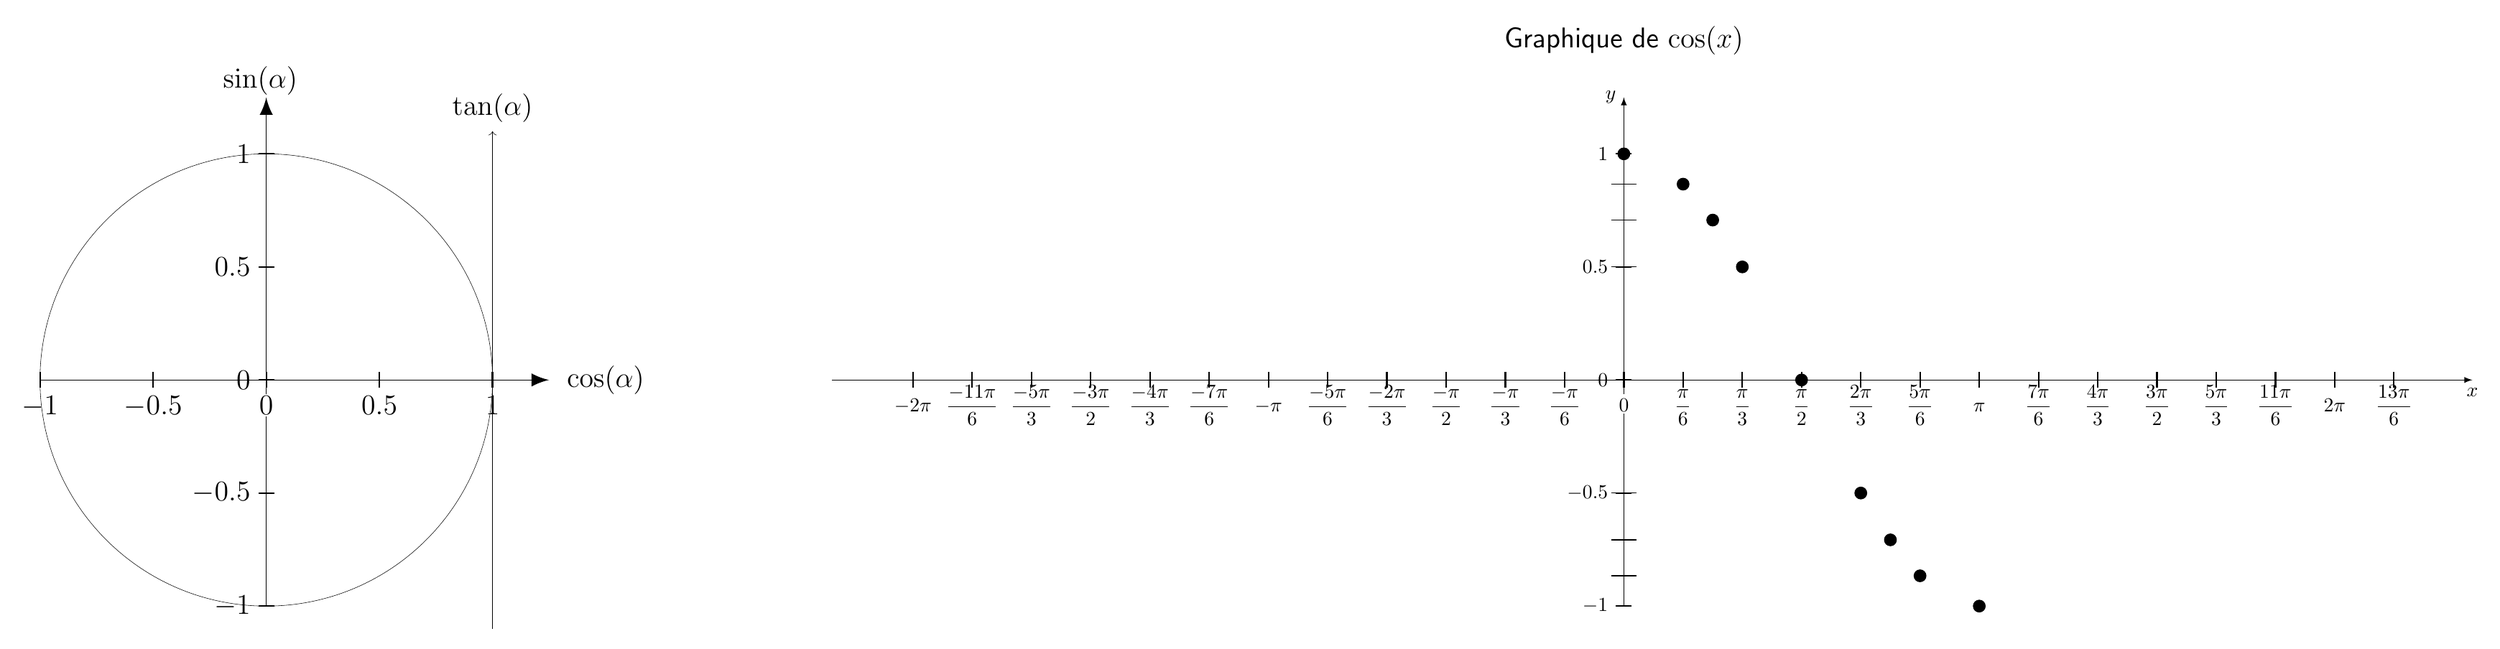
\begin{tikzpicture}[scale=2]

   \tkzInit[xmin=-7,xmax=7,ymin=-1,ymax=1, ystep=0.5]
\tkzAxeY
\tkzAxeX[trig=6]
 \tkzDefPoints{0/0.5/S1,0/0.70710678118/S2,0/0.86602540378/S3}
   \tkzDrawPoints[shape=cross,size=12](S1,S2,S3)

      \tkzDefPoints{0/-0.5/S1,0/-0.70710678118/S2,0/-0.86602540378/S3}
   \tkzDrawPoints[shape=cross,size=12](S1,S2,S3)


\tkzFct[line width=2pt,domain=-7:7]{cos(\x)}

\foreach\v in {0,1,...,6}
{
\tkzDefPointByFct[]({\v*\FPpi/6})\tkzGetPoint{A}\tkzDrawPoint[size=6](A)
}
\foreach\v in {1,3}
{
\tkzDefPointByFct({\v*\FPpi/4})\tkzGetPoint{A}\tkzDrawPoint[size=6](A)
}
\tkzText(0,1.5){\Large Graphique de $\cos(x)$}
\begin{scope}[xshift=-12cm]
   \tkzInit[xmax=1.,ymax=1.,xmin=-1. ,ymin=-1,xstep=0.5,ystep=0.5]
   \tkzDrawY[label=$\sin(\alpha)$, above, font=\Large]
   \tkzLabelY[node font=\Large]
   \tkzLabelX[node font=\Large]
   \tkzDrawX[label=$\cos(\alpha)$, right=8pt, font=\Large]
   \tkzDefPoints{0/0/O,1/0/A}
   \tkzDrawCircle[color=black](O,A)
   \tkzDefPoints{1/1.1/A,1/-1.1/B}
   \tkzDrawSegment[<-](A,B)
\tkzLabelSegment[line width=2pt, above, pos=0](A,B){\Large$\tan(\alpha)$}

\end{scope}

 \end{tikzpicture}

\end{document}
